\graphicspath{{./Ch5-SOM/images/}}

\chapter{Performance Improvement of SOM by using Low Bit-Width Resolution} \label{chap:SOM}
One of the prime reasons for NNs popularlity in last decade is due to their ability to detect pattern accurately. Compared to conventional solution they scale exceptionally well because of their inherit parallelism and are faster. NNs are also very power efficient, since their power consumption during the inference (recall) mode is very low. Apart from the NN benefits that we describe before, the main strength of the NNs comes from their ability to learn the classification criteria directly form the input data. In essence a NN trained with genomic data compresses its inputs and encodes it in its structure. The NN then can act as a predictor that can be queried about specific features in a given genome, instead of attempting to output linear DNA sequences as done in the conventional assembly. In other words, the ANN can invent an algorithm automatically that otherwise would have to be developed by the bioinformatics engineers. The algorithm is defined by the parameters of the networks, as they are developed during its training. That also provides with the possibility of retaining the network in order to update the identification features such as mutations and other genomic alterations that were not known before, without changing the algorithm itself.

Prior work in \cite{Yang2018RiBoSOM} has introduced Self-organizing maps (SOM) for rapid genome identification. SOM uses a type of unsupervised learning called competitive ANN learning model. The model reduces the data dimensions and it clusters similar data together \cite{Kohonen2013}. A trained SOM network does not require to go through the whole DNA sequence to recognize the pathogen, but only requires a small part of its DNA. SOM can be highly parallelized and such parallel implementation have been proposed for synchoros VLSI design, custom FPGA and GPUs \cite{Yang2018RiBoSOM, Porrmann2006, McConnell2012}. Another important aspect of SOM and other NNs is their robustness. NNs have been proven to work with low bit resolution without sacrificing much of their accuracy \cite{8056820}. In this work, we explore the limits of the SOM using different bit resolutions and the effect that it has on the accuracy of the SOM, as well as the benefits that this low resolution can provide for a hardware architecture. 

\section{Introduction}
An emerging design paradigm that is able to achieve better energy efficiency by trading off the quality (e.g., accuracy) and effort (e.g., energy) of computation is approximate computing~\cite{Zhang2014}. Many modern applications, such as machine learning and signal processing, are able to produce results with acceptable quality despite most of the calculations being computed imprecisely~\cite{Ye2013}. The tolerance of imprecise computation in approximate computing to acquire substantial performance gains is the basis for a wide range of architectural innovations~\cite{Esmaeilzadeh2012}. It has been demonstrated that high-precision computations are often unnecessary in the presence of statistical algorithms~\cite{Moons2017,Zhang2015}. Zhang et.al.~\cite{Zhang2015} report less than 5\% of quality loss obtained by simulation of the real hardware implemented in a 45nm CMOS technology.

Representing data with reduced bit-widths by trading off accuracy is one of the popular low-power strategy. The benefit of using reduced bit-width is improved energy performance. This is because there is a reduction in the energy cost consumption for data transfers, which usually dominates the total energy consumption for such systems.

Gupta et al. present results where they train deep networks with 16 bits fixed-point number representations and stochastic rounding~\cite{Gupta2015}. Talathi et al. show that the best performance with reduced precision can be achieved with 8 bits weights and 16 bits activation, which, if reduced to 8 bits, results in a 2\% drop in accuracy~\cite{lin2016overcoming}. Hashemi et al. look at a broad range of numerical representations applied to ANNs in both inputs and network parameters and analyze the trade-off between accuracy and hardware implementation metrics, and conclude that a wide range of representations is feasible with negligible degradation in performance~\cite{Hashemi2017}.

We present a design space exploration of a self-organizing map (SOM) to analyze the impact of different bit resolutions on the accuracy, as well as its benefits. SOM uses a type of unsupervised learning called the competitive ANN learning model. To lower the energy consumption, we exploit the robustness of SOM by successively lowering the resolution to gain efficiency and lower the implementation cost. We do an in-depth analysis of the reduction in resolution vs. loss in accuracy. We present an FPGA implementation of SOM aimed at a bacterial recognition system for battery-operated clinical use where the area, power, and performance are of critical importance. Using this implementation, we demonstrate that a 1\% loss in accuracy with 16-bit representation can yield significant savings in energy and area.
\section{Background}
In this section, we briefly introduce the SOM algorithm in \cite{Yang2018RiBoSOM} which has been used to recognize bacterial genomes.

As shown in figure \ref{fig:algorithm}, a SOM network is organized in a circle to better match genomic data. Each SOM network hosts $N$ neurons. Each neuron has a weight vector which has the same size as the training vector, assume it's $M$. Therefore, the weight matrix for the whole SOM network would be $W=M \times N$. Input sequences, either for training or for inference, are vectors of size $M$. Each element in those input vectors represents a nucleotide.
\begin{figure}[htb]
	\centerline{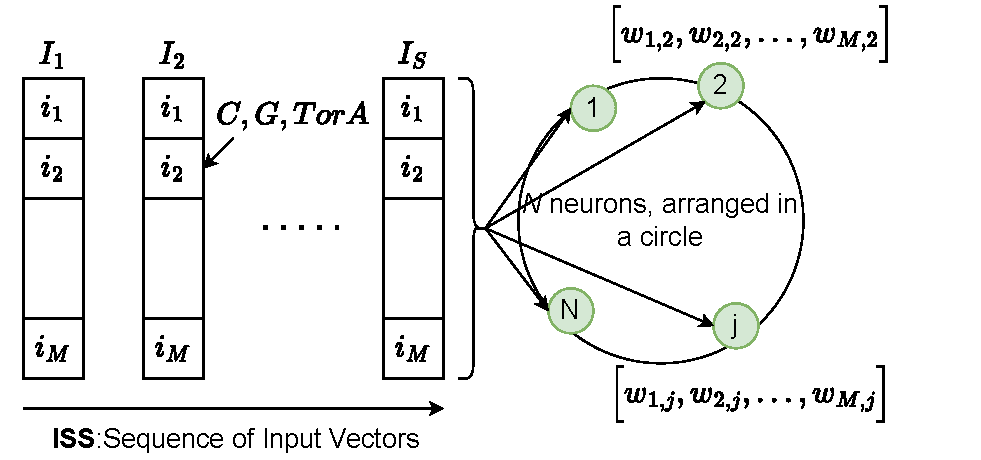
\includegraphics[width=0.5\textwidth]{SOMCircular.pdf}}
	\caption{SOM based Genomic Identification}
	\label{fig:algorithm}
\end{figure}

The actual training and inference processes are described in algorithm \ref{alg:algorithm}. The objective is to embed genomic features of a specific bacteria into a SOM. When DNA sequences of unknown bacteria are compared with trained SOM networks, the SOM network trained with the same bacteria as the unknown test bacteria, must have the highest correlation. Based on the correlation, we can identify the unknown bacteria.

The training phase is for a specific bacterial genome. The complete bacterial DNA sequence is chopped randomly into a set of fixed size training sequence, the $IS$ in algorithm \ref{alg:algorithm} line~\ref{IS_Def}. The weight matrix is initialized by random weights. On the line~\ref{beta_init}, a parameter $\beta$, initialized to 1.0, is used to control the converging process of SOM. In line~\ref{dist_min} and~\ref{j_min}, the actual training process first tries to find the neuron that best matches the particular input vector. Then, weights of the neighbourhood of the winning neuron are updated based on the distance between the target neuron and the winning neuron, as shown in line~\ref{dist_update} and~\ref{W_update}. Finally in line~\ref{beta_update}, the parameter $\beta$ is decreased by a factor. After repeating the training process for all training vectors, the SOM will learn the features of that particular bacterial genomes. Each SOM network can be trained to recognize only one bacteria. In order to recognize a range of bacteria, many SOM networks need to be trained.

During test phase, some test DNA fragments from one unknown bacteria are send to each trained SOM network. The SOM network that correlates the test input sequence best, is chosen as the winning SOM and the bacteria it represents reveals the identity of the unknown test bacteria. The correlation measurement is marked by the score shown in line~\ref{score}. The smaller the score is, the better it correlates with the input test vectors.
\begin{algorithm}[htb]
	 \caption{Pseudo code SOM learning and inference for genome identification}
	\label{alg:algorithm}
	\begin{algorithmic}[1]\label{Algo:SOMTraining}
%		\Procedure{SOMTraining}{$N,I,IS,W$}
		\Statex \mbox{\textbf{Algorithm Part 1}: SOM training for 1 bacterial genome}
		\Statex \textbf{Input} $N:$ Number of neurons
		\Statex \textbf{Input} $I{=}[i_1, i_2, ..., i_M]$: Input-Vector
       	\Statex \textbf{Input} $IS{=}{I_1, I_2, ..., I_S}$: Sequence of Input-Vectors, each IS represents one bacterial genome\label{IS_Def}
       	\Statex \textbf{Input} $W_{i,j}: M\times N$ weight matrix for 1 bacteria
        \State $\beta_{min}=0.01$; $decay\_factor=0.99$; $\beta=1.0$\label{beta_init}
		\For{$I_k \in IS$}
		\State $dist_{min}=\min\limits_{j=1...N}(\sum_{i=1}^{M}|I_{k,i}-W_{i,j}|)$\label{dist_min}
        \State $j_{min} = j$ where $dist_{j} = dist_{min}$\label{j_min}
        \For{$j \in 1...N$}
           \State $dist = \frac{N}{2} - ||j-j_{min}|-\frac{N}{2}|$\label{dist_update} \Comment{toroid distance}
           \State $W_j = W_j - \frac{\beta}{2^{dist}}(W_j-I_k)$\label{W_update}
        \EndFor
        \State $\beta = \min(\beta*decay\_factor, \beta_{min})$\label{beta_update}\Comment{decay $\beta$}
		\EndFor
%		\EndProcedure
%    \Procedure{SOMInference}{$N,I,IS,W$}
  \Statex
   \mbox{\textbf{Algoritm Part 2}: SOM inference}
    \Statex \textbf{Input} $TIS{=}{I_1, I_2, ..., I_S}$: Test Input Sequence of Input-Vectors for which the bacteria is to be identified
    \Statex \textbf{Input} $W_{r,j,i}{=}R\times N \times M$: Weights for R bacteria
    \State $Inferred\_r$ is $r$ with\label{inferred_r}
    \State $score{=}\min\limits_{r=1...R}\Bigl[\sum_{k=1}^{S}\min\limits_{j=1...N}(\sum_{i=1}^{M} |I_{k,j}-W_{r,i,j}|)\Bigr]$\label{score}
%   \EndProcedure		
	\end{algorithmic}
\end{algorithm}
\section{Low bit-width FPGA Design of SOM}\label{custom}
In this section, we present the FPGA implementations that were used to implement SOM for identification of bacterial genomes. The FPGA implementation is done on Xilinx Virtex7 485t chip for the identification of bacterial genomes. 

A custom semi systolic array was hand crafted, for different bit width implementations, to analyze the area versus energy trade off. The design takes a vector of weights as input and finds the neuron in the network closest to input vector. This neuron is referred as winning neuron of the network. The design outputs the distance between the input vector and closest neuron's weights vector. This distance or score is used for identifying the bacteria in the test samples. During the training phase neurons weights are updated according to their distances from the winning neuron.
\begin{figure}[h]
	\captionsetup{font=sf}
	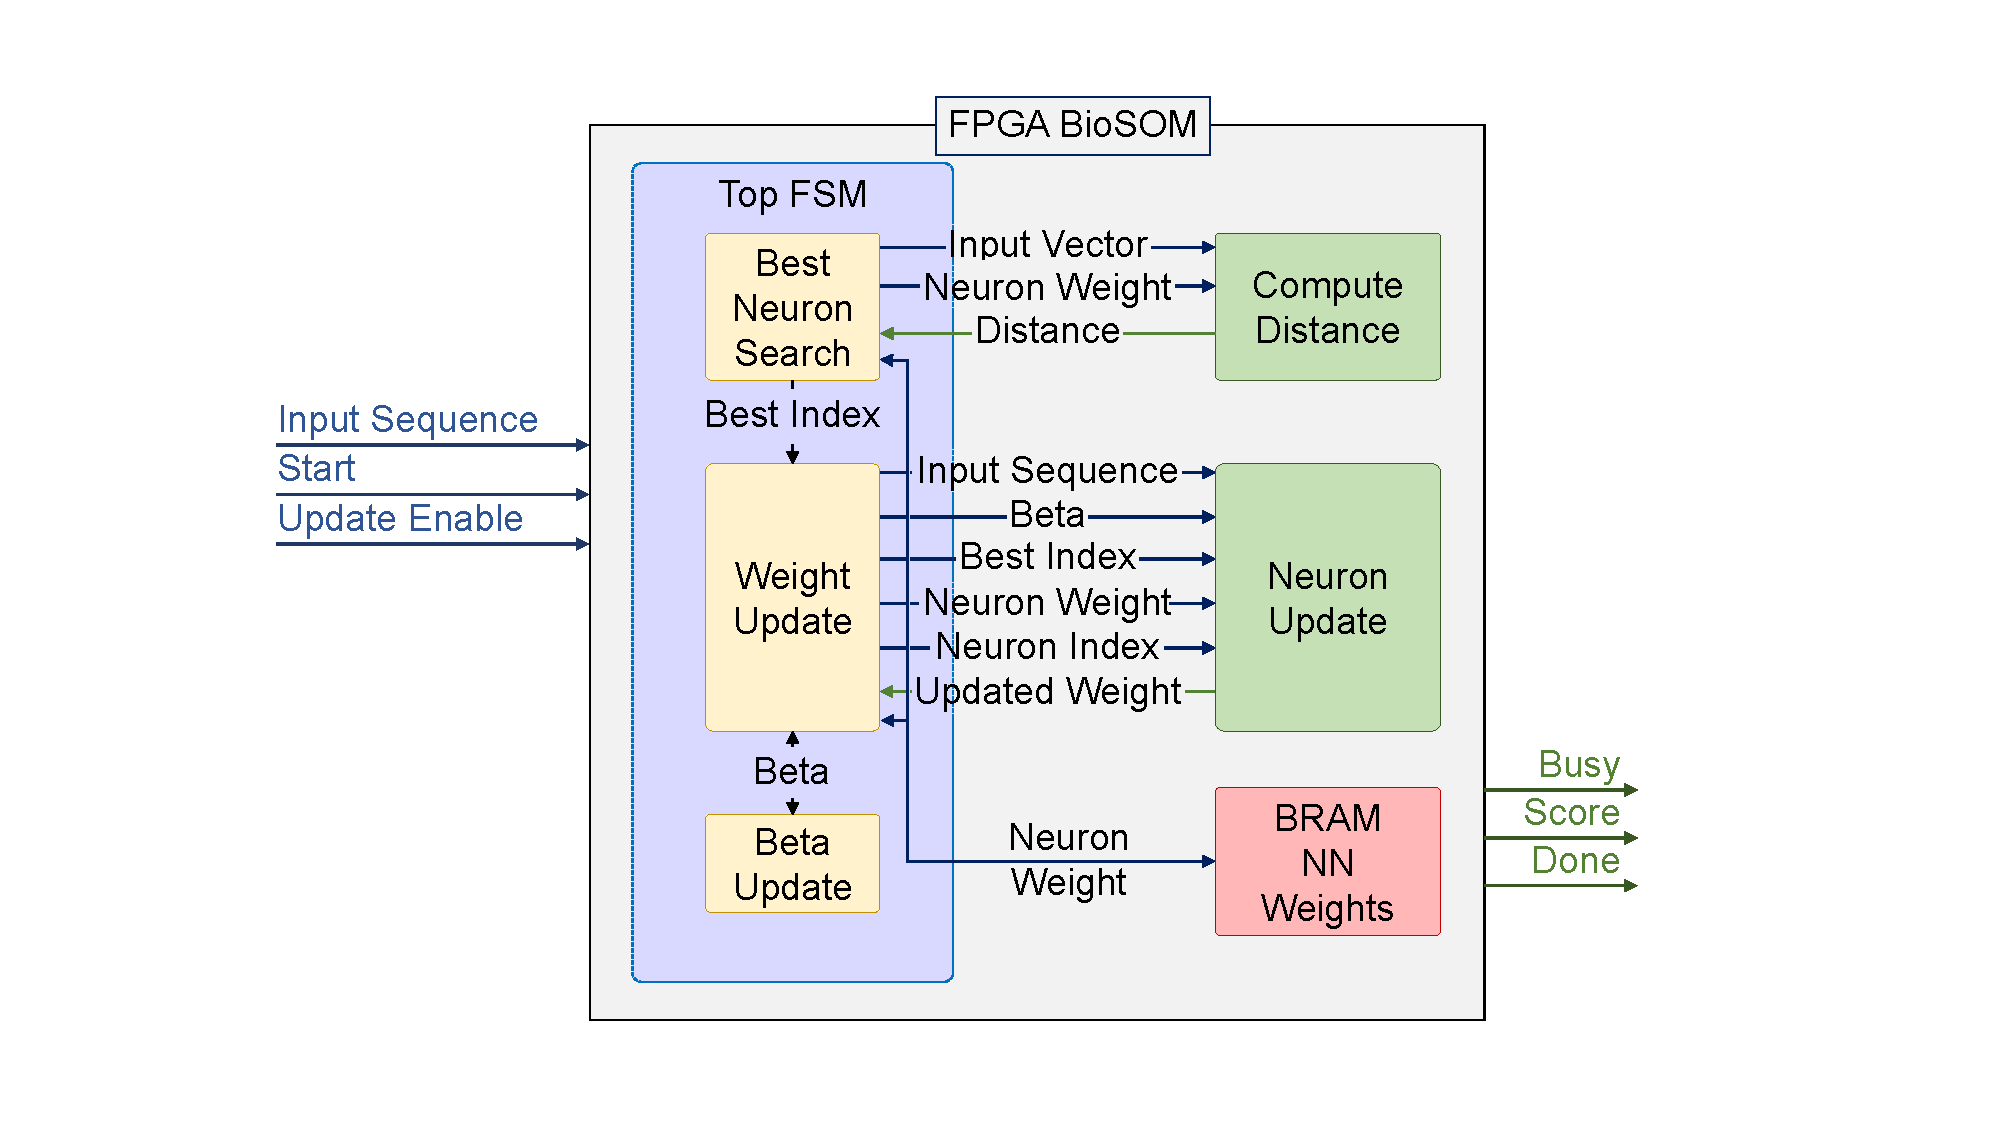
\includegraphics[width=0.65\columnwidth]{SOMDesignOne_v2}
	\caption{Hardware Module for BioSOM.}
	\label{fig:SOMFPGAImplementation}
\end{figure}
Figure \ref{fig:SOMFPGAImplementation} shows a high level schematic of the FPGA implementation of BioSOM and illustrates the key components in the design. The input is a $n$-bit vector. Each pair of bits in the input represents one of nucleotide A,C,G or T. Thus a 16-bit word contains 8 symbols. 

The Neural Network weights are stored in 2-dimensional array in BRAMs. $1^{st}$-dimension represent neurons in the network and $2^{nd}$-dimension holds the weights of each neuron. Each neuron has 8 weights and each weight is stored as a fixed-point number. Bit width analysis is performed by varying the number of bits (8, 12, 16, 24 and 32) used to represent the weights.

During testing phase, only \textit{Compute Distance}, Figure \ref{fig:ComputeDistance}, is enabled (\textit{Update Enable=0}). This component returns the distance of a neuron from input weights. Using this distance, winning neuron of the network is identified.
This component has pipe-lined implementation with an Initiation Interval (II) equal to 1. Each stage of the pipeline computes the difference between one input weight and corresponding neuron weight and updates the input partial sum. Output of each stage is fed as partial sum into next stage. Last stage output is the distance between the input and neuron.
\begin{figure}[h]
	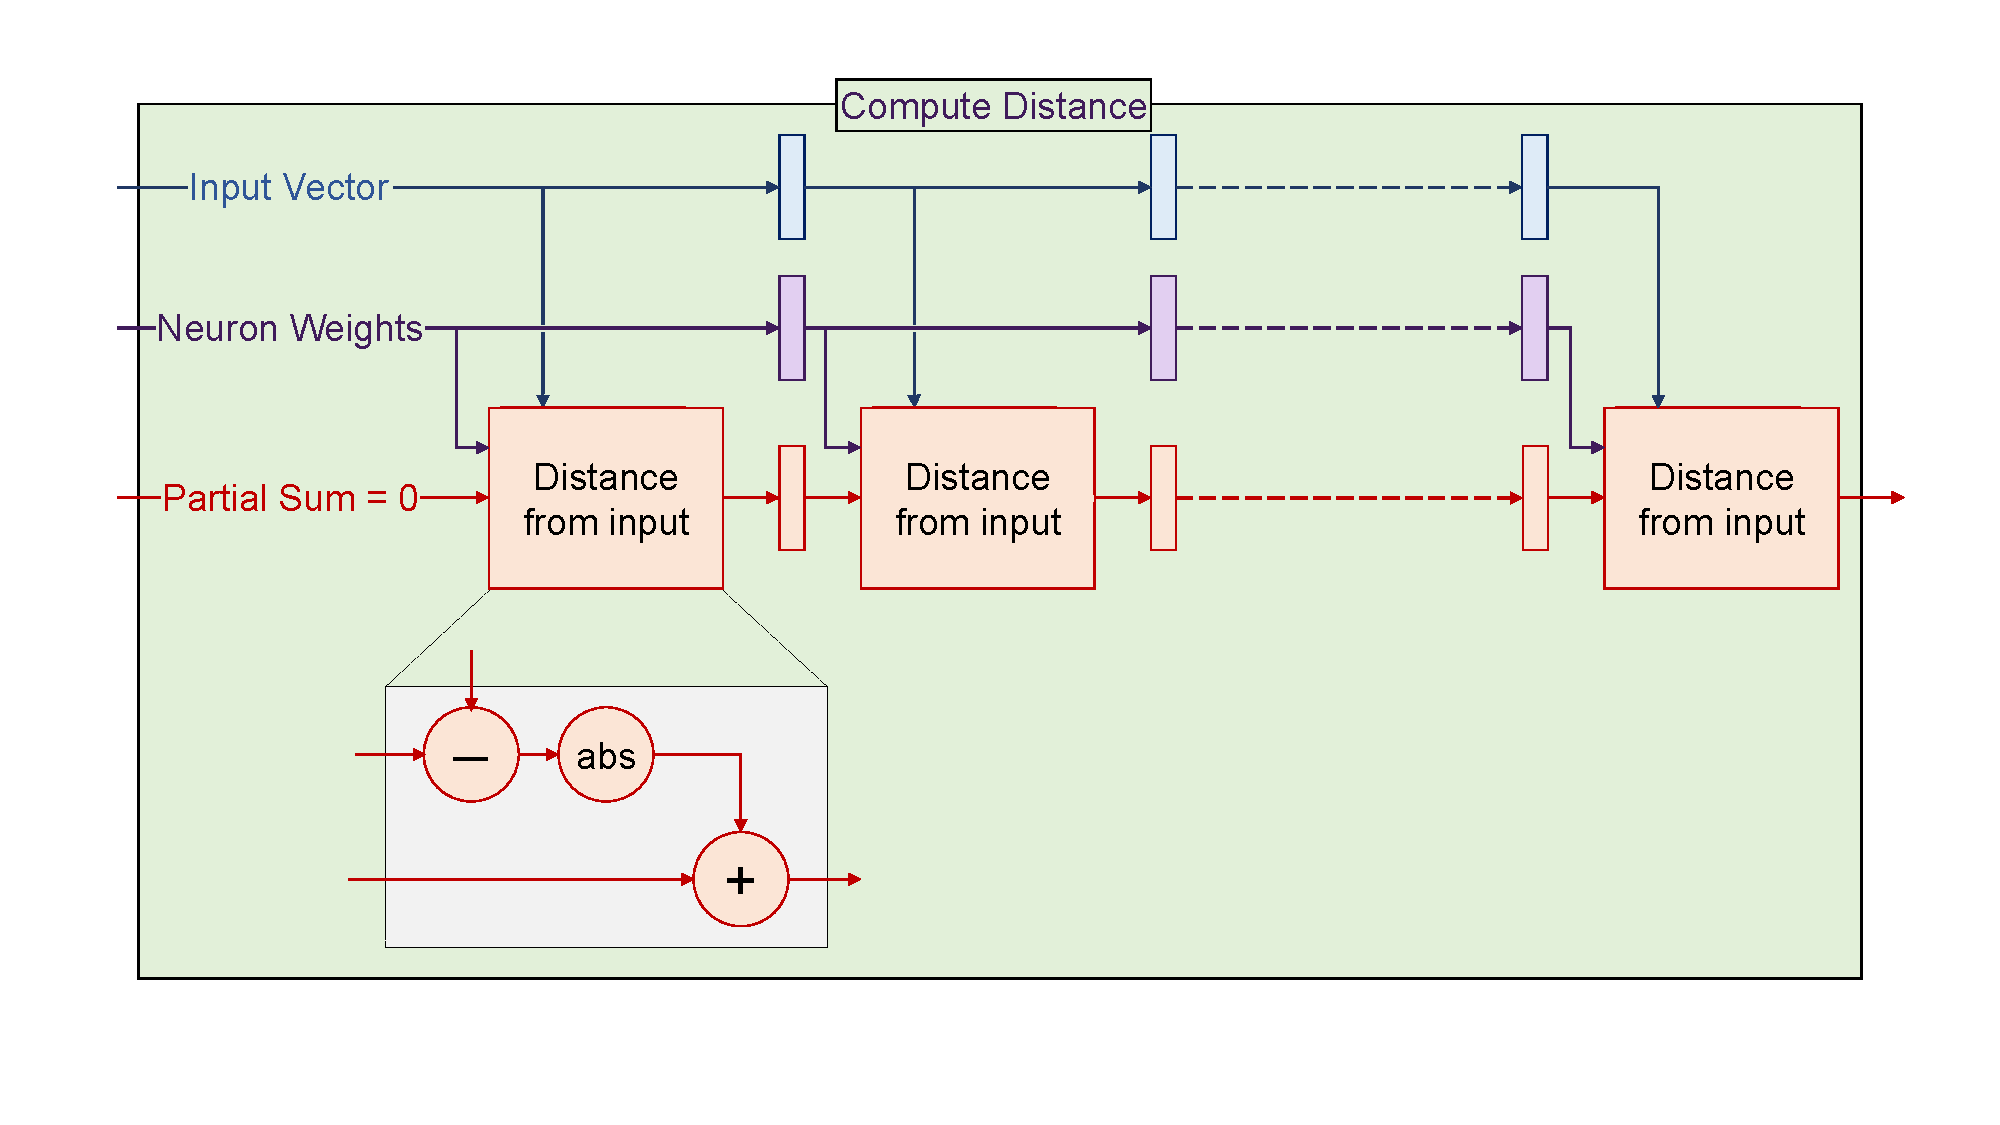
\includegraphics[width=0.65\columnwidth]{computeDistance_v2}
	\caption{Compute Distance Module.}
	\label{fig:ComputeDistance}
\end{figure}

During training phase \textit{Neuron Update} component is enabled by setting (\textit{Update Enable=1}). The weights of the Neurons are updated using the distance output of the \textit{Compute Distance} module. The \textit{Neuron Update} component is also pipe-lined design with II=1. The stages of pipeline are shown in Figure \ref{fig:NeuronUpdate}.
\begin{figure}[h]
	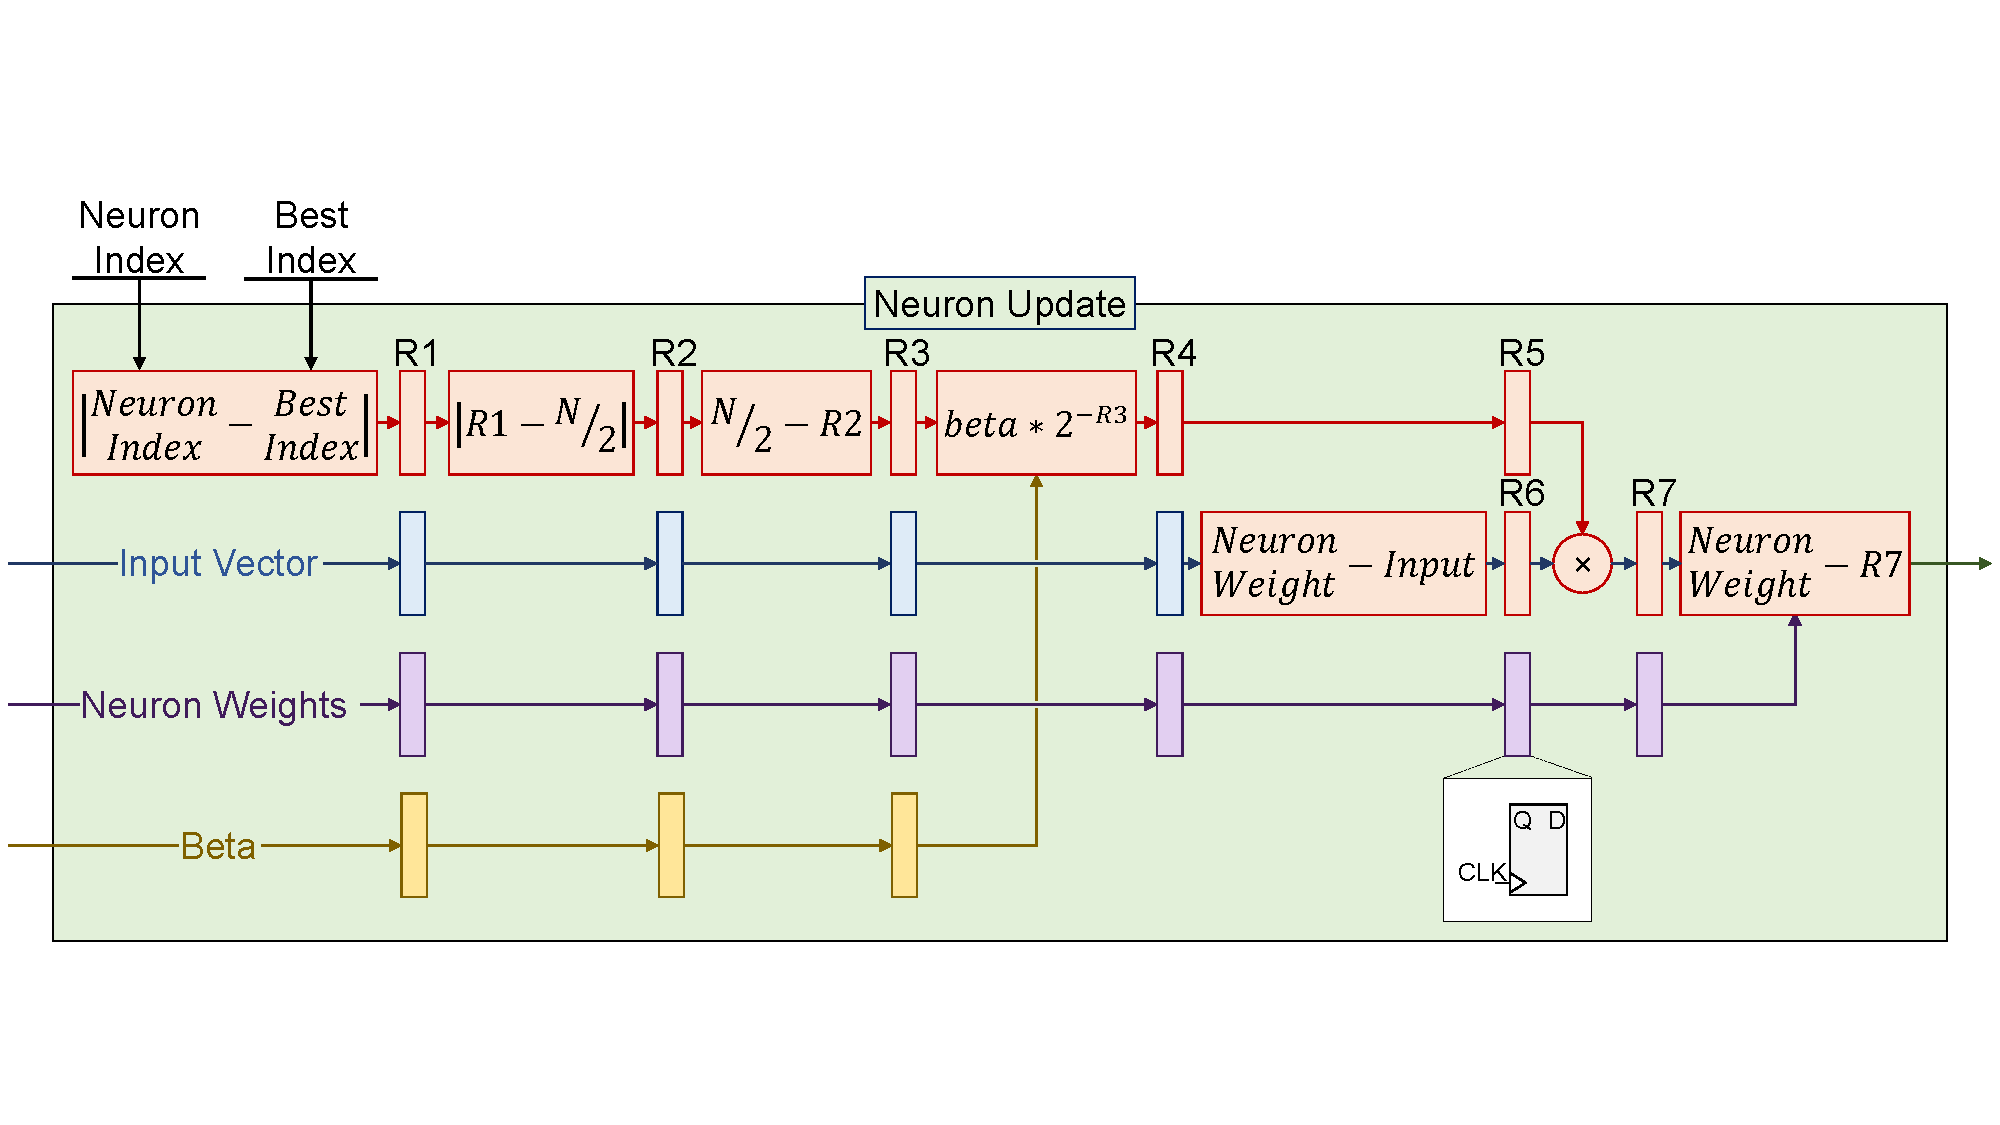
\includegraphics[width=0.65\columnwidth]{neuronUpdate_v2}
	\caption{Neuron Update Module.}
	\label{fig:NeuronUpdate}
\end{figure}

Clearly, the \textit{Neuron Update} can only start after \textit{Compute Distance} has completed finding closest neuron. So these two components can execute sequentially for a given input vector. However, while \textit{Neuron Update} is updating the weights for an \textit{Input Vector=i}, \textit{Compute Distance} can start its operations for next \textit{Input Vector=i+1}.  \textit{Compute Distance} and \textit{Neuron Update} components can overlap their execution, processing different input vectors at same time. This design has overall ${II=23+N}$ cycles, where N is number of neurons in the network.

\section{Experimental Results And Analysis}\label{sec:results}
In this section we present the results from our experiments. In subsection \ref{ex_setup} we give the details of our experimental setup used for measuring the accuracy of the SOM. Subsections \ref{fpga_results} describe the experimental setup and presents the results of the FPGA implementation.
\subsection{Accuracy experimental setup}\label{ex_setup}
The SOM has been implemented with a range of fixed-point formats. With fewer bits, one naturally expect that the SOM network for bacterial identification to suffer from accuracy degradation. A MATLAB simulation model was created to analyze the accuracy loss when using fixed-point implementation. The experiment used a scaled down version of bacterial identification problem, to reduce the training time of the network. We consider that this does not compromise the resulting accuracy of the SOM. We trained 10 SOMs with 10 different bacteria DNA sequences. Each SOM network has 100 neurons inside, and each neuron has 20 weights. We trained the networks by two independent training processes running in parallel. One is implemented using double precision floating point and the other is implemented with fixed-point weights. After training, we used the trained networks to identify the unknown sequence and record their scores.

Two metrics are defined to evaluate the implementation accuracy. The \emph{quantization error} is defined as the relative error between fixed-point format score ($S_{fixed}$) and double precision floating-point format score ($S_{float}$):
\begin{align*}
	quantization\_error = \frac{|S_{fixed} - S_{float}|}{S_{float}}\times 100\%
\end{align*}
The \emph{classification error} is defined as the ratio of the number of times the network classified ($C_{false}$) the bacterial strain to the total number of tests performed ($C_{total}$):
\begin{align*}
	classification\_error = \frac{C_{false}}{C_{total}}\times 100\%
\end{align*}
Classification error and quantization error are not completely independent, but they reveal the different aspects of fixed-point implementation accuracy. Quantization error shows the difference between fixed-point representation and golden double point reference. It doesn't change with the problem. Classification error determines the final impact of the accuracy loss introduced by the fixed-point implementation, and is problem dependent. Figure \ref{fig:error} presents the quantization error and the classification error depending on the bit resolution. From the figure, 8-bit representation completely fails the experiment, 12-bit has 39\% classification error, 16-bit has $<$1\%, 24-bit and 32-bit successfully pass the experiment with 0\% of classification error. However, we should notice that though 16-bit pass the test, it still has about 10\% quantization error.\par
\begin{figure}[ht]
	\centering
	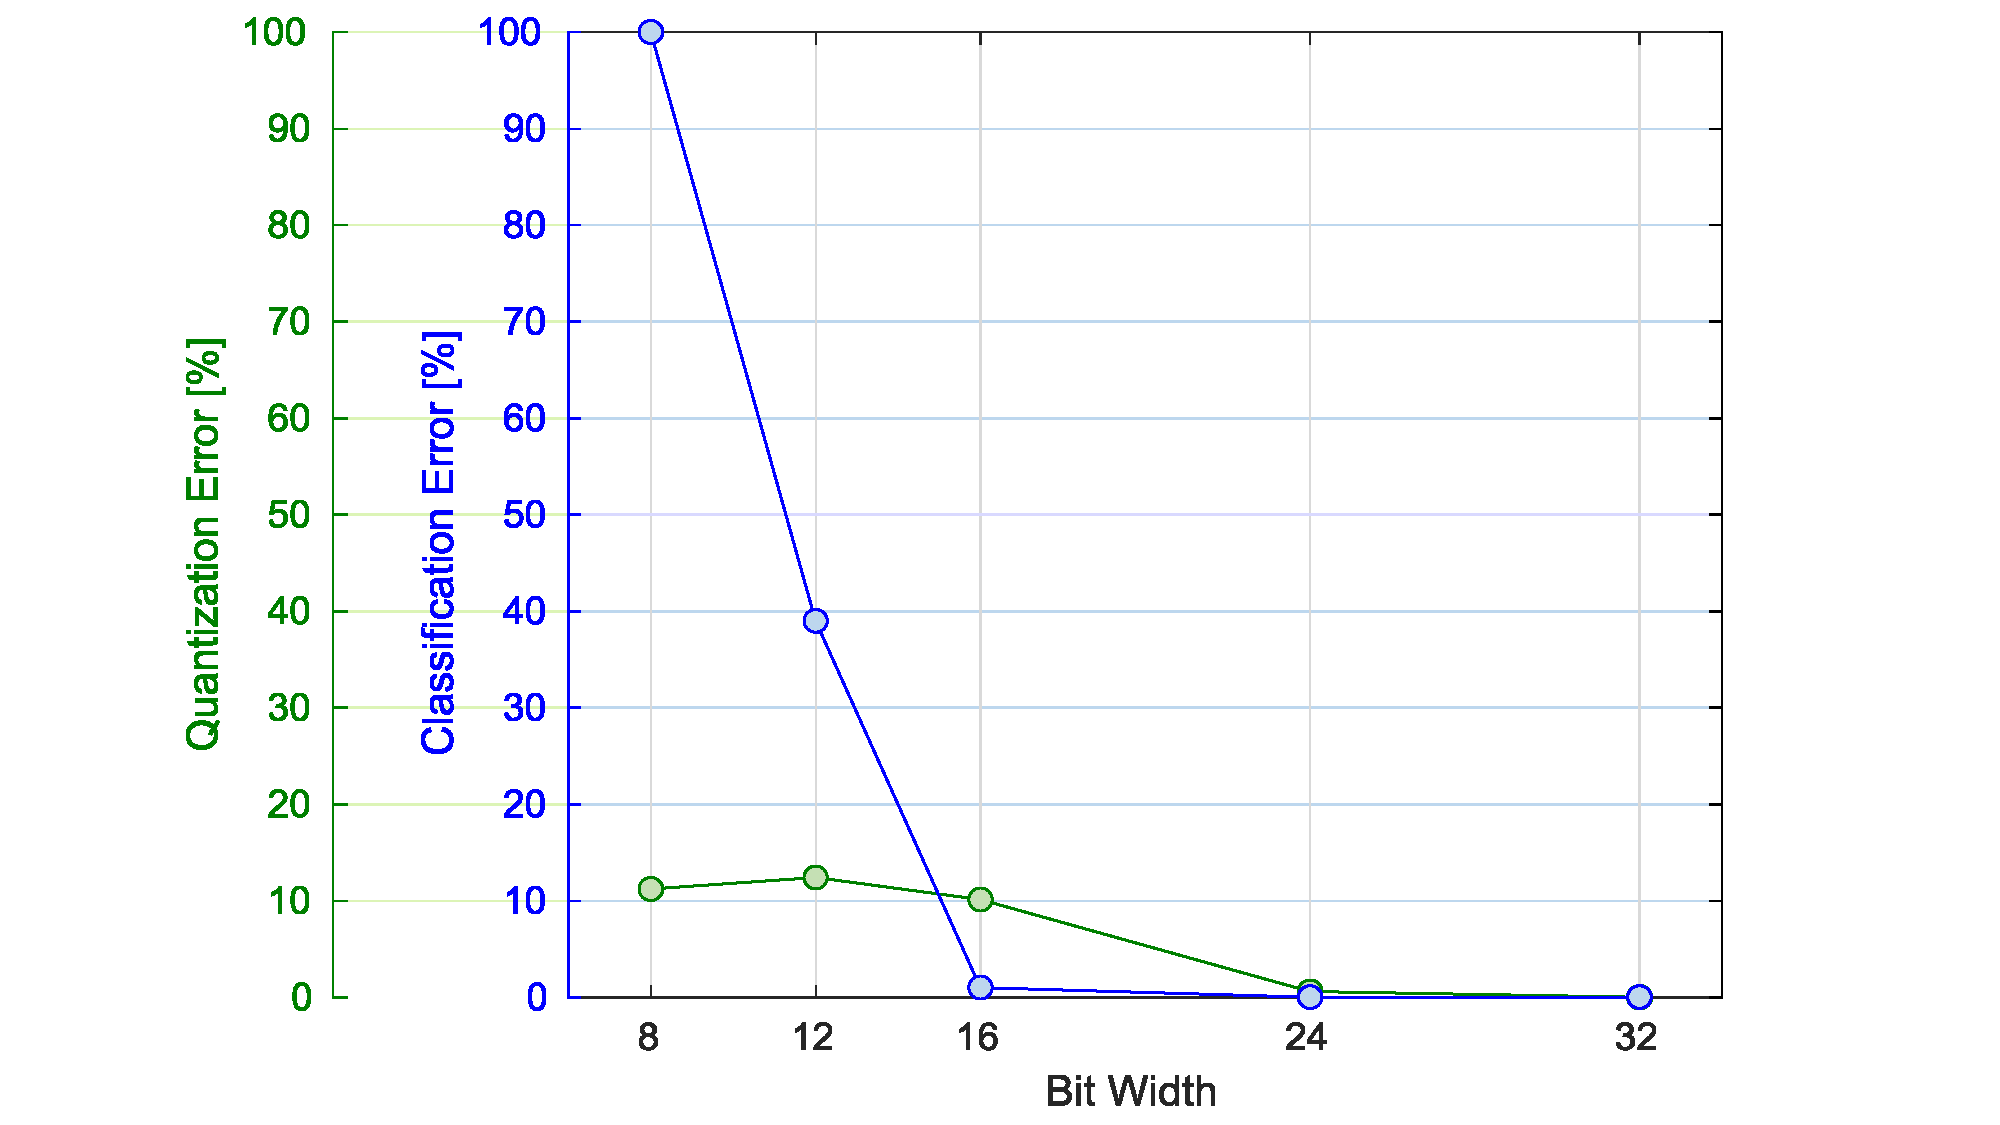
\includegraphics[trim=  85 5 130 8, clip, width=0.45\columnwidth]{accuracy}
	\caption{Quantization error compare to the identification error}
	\label{fig:error}
\end{figure}
We like to note that each SOM was trained with the specific fixed-point resolution and that the quantization error shows the difference of the \emph{score} variable, see algorithm \ref{alg:algorithm}, between the fixed-point and the double precision. The quantization error is very important for the \emph{score} variable of the SOM, since this variable is the one that decides which is the winning SOM, i.e. which SOM matches the input DNA sequence. It is important to guarantee sufficient bits for the \emph{score} of each SOM. If the resolution is too low, the \emph{score} of the SOMs after quantization will be identical even with low quantization error which makes it impossible to identify the bacteria correctly. This explains the fact that in Figure \ref{fig:error} the quantization error is low but the classification error is high in 8 to 12-bit resolution region.
\subsection{FPGA experimental setup}\label{fpga_results}
In this section we present the experimental results of the FPGA implementation presented in section \ref{custom}. The FPGA design is implemented with Vivado v.2016.4 used for synthesis and analysis of the HDL Designs. Our design is implemented in VHDL and validated using the Vivado simulator. Experimentation is done for different fixed point representations of weights by modifying parameters in VHDL code. 
\begin{figure*}[hb]
	\centering
	\subfloat[FPGA LUT utilization]{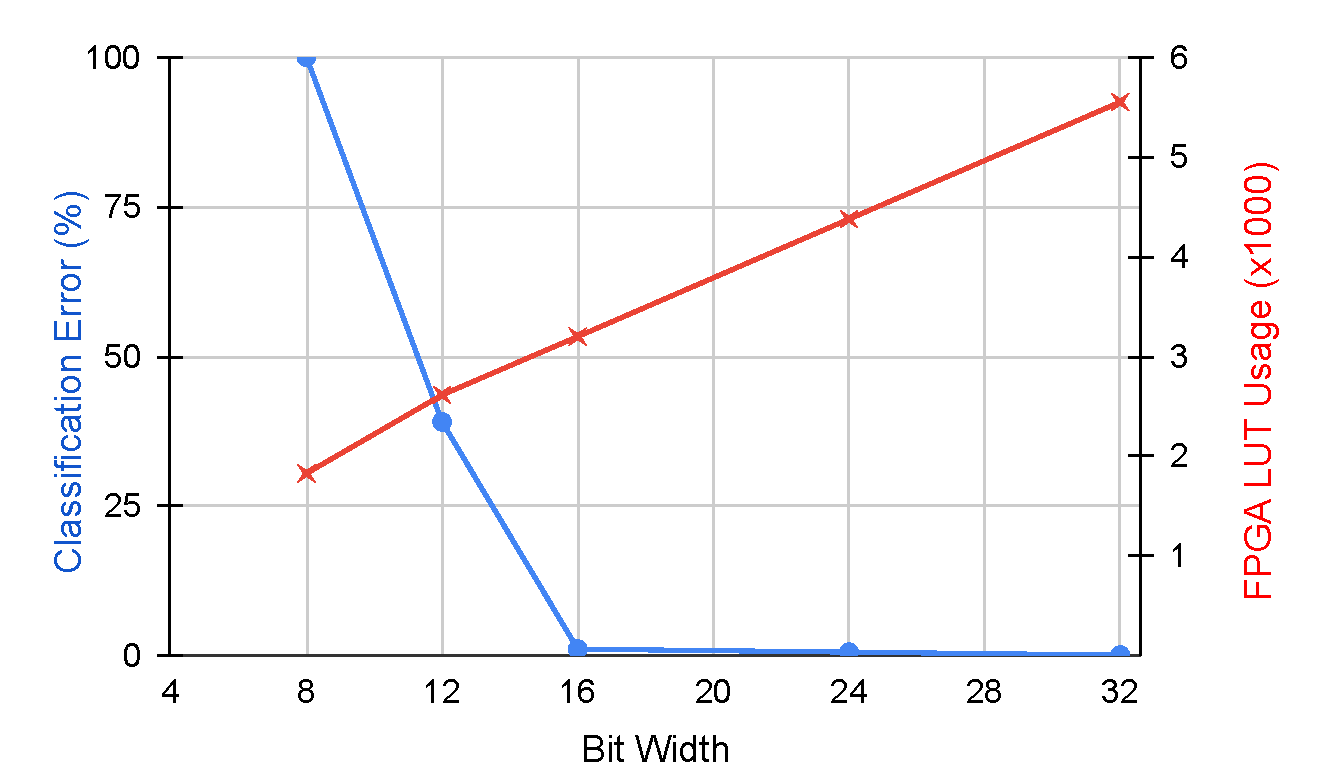
\includegraphics[width=0.45\columnwidth]{area}
		\label{fig:area}
	}~
	\subfloat[energy of FPGA implementation]{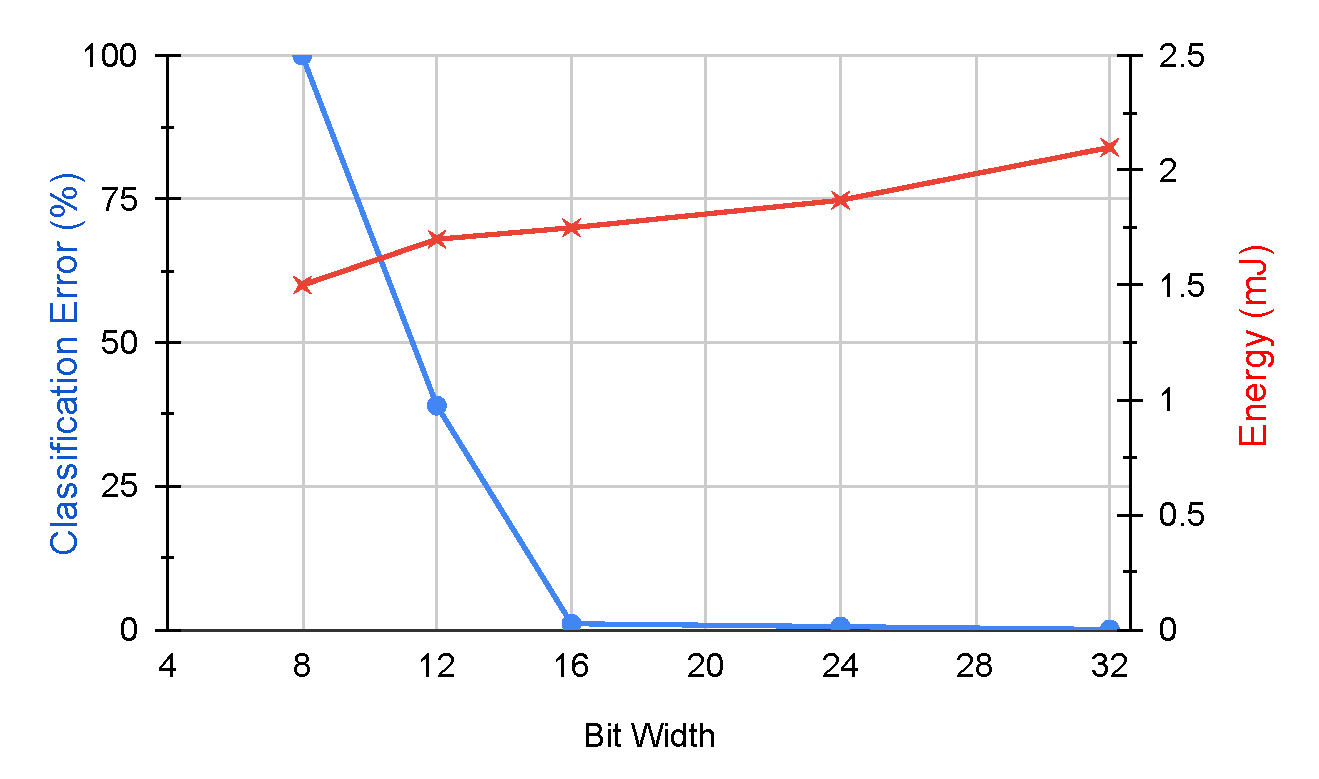
\includegraphics[width=0.46\columnwidth]{energy}
		\label{fig:energy}
	}
	\caption{ Area and energy comparison for different fixed-point format.}
	\label{fig:metrics}
\end{figure*}

The area and power numbers for different weight resolutions are extracted from the reports generated by Vivado tool post placement and routing with a working frequency of 100 MHz.
Table \ref{table:1} compares the resources and area for 8, 12, 16, 24, and 32 bits fixed point formats, for a SOM network with 512 neurons. The second part of the table compares the average power in the different fixed point formats, for the same SOM.

\begin{table}[h!]
	\centering
	\caption{Resource Comparison of different fixed point formats}
	\label{table:1}
	\begin{tabular}{ c |c | c| c |c | c } 
		\toprule
		Resource & 8b & 12b & 16b & 24b & 32b \\ 
		\midrule
		LUTs & 1823 & 2611 &3196 & 4375 & 5549 \\
		\hline
		Registers & 3481 & 4679 & 5871 & 8255 & 10639 \\ 
		\hline
		Slice & 854 & 1158 & 1369 &1809 & 2395 \\ 
		\hline
		LUT FF Pairs & 1007 & 1369 & 1750 & 2372 & 3043 \\
		\hline
		B-RAM & 4 & 6 & 8 & 11 & 15 \\
		\hline
		DSP48E1 & 17 & 17 & 17 & 17 & 33 \\
		\hline
		Bonded IOB & 57 & 61 & 65 & 73 & 81 \\
		\midrule
		%    \end{tabular}
	%\end{table}
	
	%\begin{table}[h!]
	%    \centering
	%    \caption{Power Comparison of different fixed-point formats}
	%    \label{table:2}
	%    \begin{tabular}[t]{ c |c | c| c |c | c } 
		\midrule
		Power(W) & 8b & 12b & 16b & 24b & 32b \\ 
		\midrule
		Total Power & 0.295 &0.314 &0.332 &0.356 &0.392 \\
		\hline
		Dynamic &0.052 &0.071 &0.089 &0.113 &0.148 \\ 
		\hline
		Device Static &0.243 &0.243 &0.243 &0.244 &0.244 \\ 
		\bottomrule
	\end{tabular}
\end{table}
The results are summarized in the Figure \ref{fig:area} and \ref{fig:energy}. Both the amount of utilized LUTs and total energy in Joule is presented against the classification error. From the figures, we can easily conclude that, we can substantially reduce the resources used and the energy by using a 16-bit fixed-point representation, without losing accuracy. We can reduce the resources even further by moving to the 12-bit representation, by sacrificing 39\% of the SOM accuracy. 
\section{Summary}
In this work we explore the design space of a self-organizing map (SOM) used for rapid and accurate identification of bacterial genomes. This is an important health care problem because even in Europe, 70\% of prescriptions for antibiotics is wrong.  The  SOM is trained on Next Generation Sequencing (NGS) data and is able to identify the exact strain of bacteria. This is in contrast to conventional methods that require genome assembly to identify the bacterial strain. SOM has been implemented on FPGA and shown to have better computational efficiency compared to GPUs. To further lower the energy consumption, we exploit the robustness of SOM by successively lowering the resolution to gain further improvements in efficiency and lower the implementation cost without substantially sacrificing the accuracy. We do an in depth analysis of the reduction in resolution vs. loss in accuracy as the basis for designing a system with the lowest cost and acceptable accuracy using NGS data from  samples containing multiple bacteria from the labs of one of the co-authors. The objective of this method is to design a bacterial recognition system for battery operated clinical use where the area, power and performance are of critical importance. We demonstrate that with 39\% loss in accuracy in 12 bits and 1\% in 16 bit representation can yield significant savings in energy and area.

In this work, we implemented FPGA design for SOMs. The mapping support different bit width to enable trade-offs between accuracy and computation cost. Experiments has shown the big design space, resulting in different cost in terms of timing, area as well as energy, all of which are affected significantly by the fixed-point format representation. Through the experiment, we conclude that the SOM network with 16-bit fixed-point representation implemented on FPGA, has better benefits compared to other fixed-point formats with more bits. And 16-bit has acceptable classification error. Format with bits more than 16 no longer add any benefit to lower the classification error. 

In future works, we plan to apply more sophisticated methods to scale down the bit width without losing too much accuracy. For example, the weights can be dynamically scaled after several epochs of training when the current fixed point format is not suitable anymore. We are confident that, with such approximate computing techniques, we could possible reduce the resolution to 8 bits with acceptable loss of accuracy and, by extension, the implementation cost of SOM networks on hardware.